\chapter{Experiments and Results}
In this section, computer simulation results are presented in a two-dimensional space. The scoring system for formation coordination is validated in Section 4.1. The path planning algorithm is tested via three scenarios in Section 4.2, where the first one shows how the team avoids obstacles by spitting and merging, the second one shows how the team compresses the formation to pass through a narrow passage, and the last one validates how the team finds a solution when encountering a blocked corner. The parameters used in our simulation are shown in Table \ref{table:parameter}:


\begin{center}
\captionof{table}{Simulation parameters}
\label{table:parameter}
\scalebox{0.9}{ %表格縮放
\begin{tabular}{ll} 
    \Xhline{1.3pt}
    \textbf{parameter} & \textbf{value} \\ 
    \Xhline{1.3pt}
        UAV radius ($r$) & 0.4 $m$\\
        safe distance ($d_{safe}$) & 0.8 $m$\\
        minimum velocity ($v_{min}$) & 0 $m/s$\\
        maximum velocity ($v_{max}$) & 15 $m/s$\\
        maximum acceleration ($a_{max}$) & 0.3 $m/s^{2}$\\
        minimum yaw rate ($\omega_{min}$) & $-40\cdot\frac{\pi}{180}$ $rad/s$\\
        maximum yaw rate ($\omega_{max}$) & $40\cdot\frac{\pi}{180}$ $rad/s$\\
        maximum yaw acceleration ($\omega_{max}$) & $40\cdot\frac{\pi}{180}$ $rad/s$\\

        predicted time ($t_{T}$) &	2 $s$\\
        time tick  &	0.2 $s$\\
    \Xhline{1.3pt}
\end{tabular}}
\end{center}


\section{Validation of The Scoring System}

To fully verify the formation coordination's performance, we use an obstacle-free environment to observe how the UAVs move based on the scoring system. In Figure \ref{reconfiguring}, 9 random-positioned UAVs are seen in the bottom-left corner, each of which has a sensing radius $d_{r}$ of 5 meters. After taking off, as in Figure \ref{reconfiguring_a}, UAVs instantly detect the neighbors within $d_{r}$ and plan the best trajectories considered the minimum cost in the scoring system. At $t= 5 sec$ , as in Figure \ref{reconfiguring_b}, UAVs move closer among neighbors to form compactly. At $t= 10 sec$, the final formation is reconfigured as in Figure \ref{reconfiguring_c}. The final formation differs each time during multiple simulations since our goal is to present the flexible and safe behavior of the path planning algorithm. It also shows scalability with the number of UAVs in the simulation. Because $N$ does not affect the visual scope, each UAV only has to consider the neighbors as its reference. 

\begin{figure}[htbp]
     \centering
     \begin{subfigure}[b]{0.3\textwidth}
         \centering
         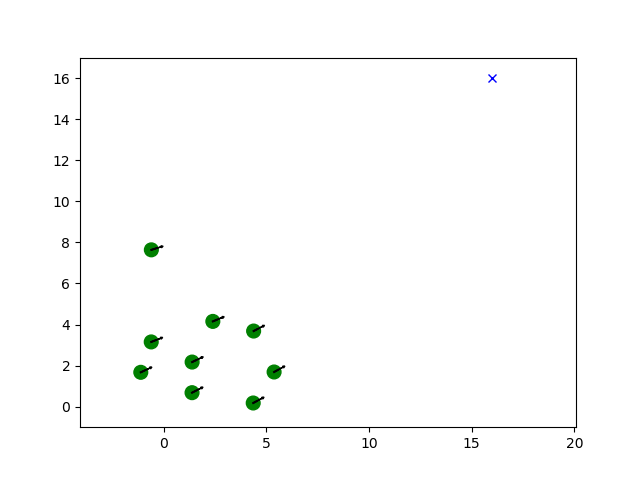
\includegraphics[width=\textwidth]{figures/reconfigure_1.png}
         \caption{random positioned UAV}
         \label{reconfiguring_a}
     \end{subfigure}
     \hfill
     \begin{subfigure}[b]{0.3\textwidth}
         \centering
         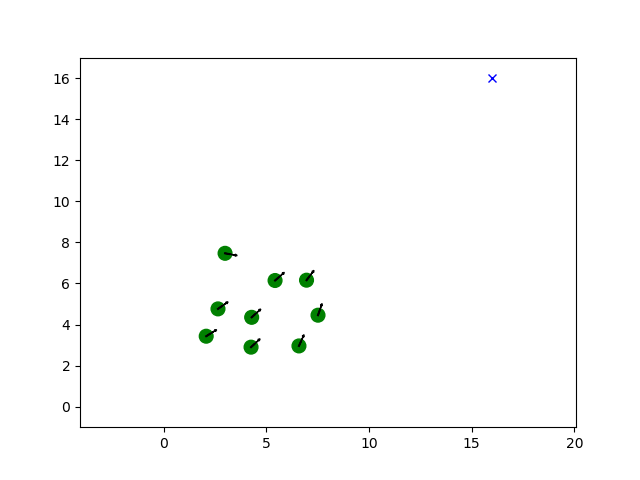
\includegraphics[width=\textwidth]{figures/reconfigure_2.png}
         \caption{formation coordination}
         \label{reconfiguring_b}
     \end{subfigure}
     \hfill
     \begin{subfigure}[b]{0.3\textwidth}
         \centering
         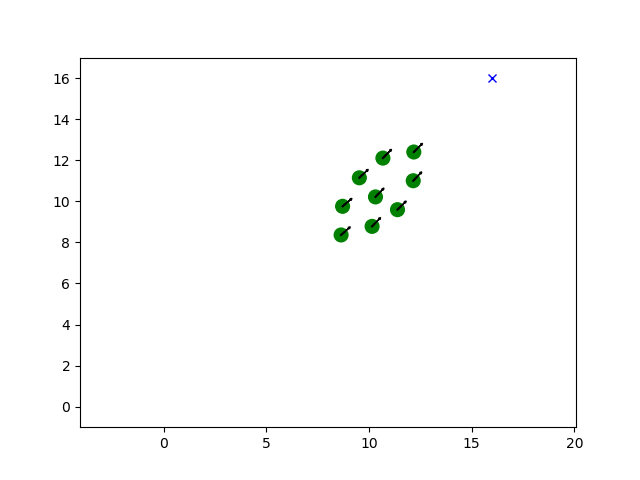
\includegraphics[width=\textwidth]{figures/reconfigure_3.png}
         \caption{final formation}
         \label{reconfiguring_c}
     \end{subfigure}
        \caption{Reconfiguring a compact formation}
        \label{reconfiguring}
\end{figure}


In the second simulation shown in Figure \ref{fig:merging}, we separate 9 UAVs into two groups and observe the behavior between them while flying toward the same goal point. At the beginning. as in Figure \ref{fig:merging_a}, two groups are initially positioned at separate locations. At $t=5$, as in Figure \ref{fig:merging_b}, several UAV's sensors in both groups detect the positions of UAVs in the other group, which they increase the number of neighbors. Therefore, the two groups merge to form a new formation into a large team at $t=17$, as in Figure \ref{fig:merging_c} . 

\begin{figure}[htbp] 
     \centering
     \begin{subfigure}[b]{0.3\textwidth}
         \centering
         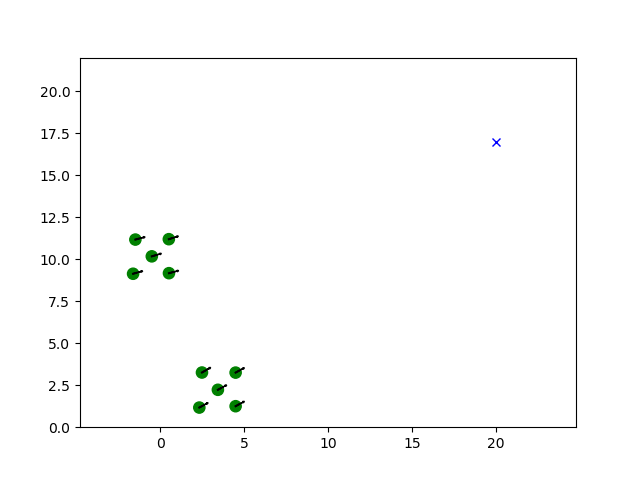
\includegraphics[width=\textwidth]{figures/merge_1.png}
         \caption{before merging}
         \label{fig:merging_a}
     \end{subfigure}
     \hfill
     \begin{subfigure}[b]{0.3\textwidth}
         \centering
         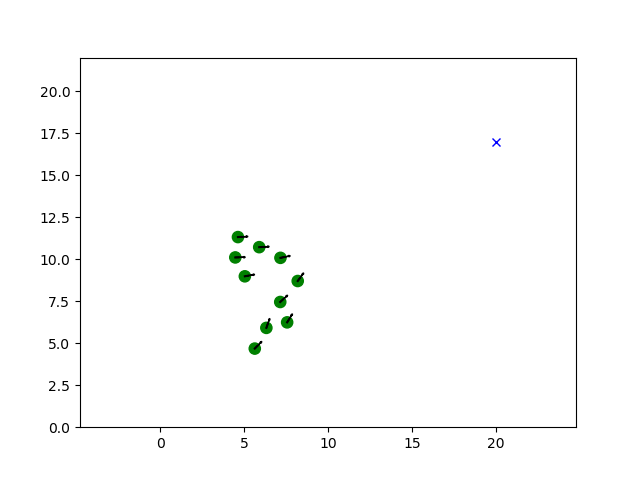
\includegraphics[width=\textwidth]{figures/merge_2.png}
         \caption{formation coordination}
         \label{fig:merging_b}
     \end{subfigure}
     \hfill
     \begin{subfigure}[b]{0.3\textwidth}
         \centering
         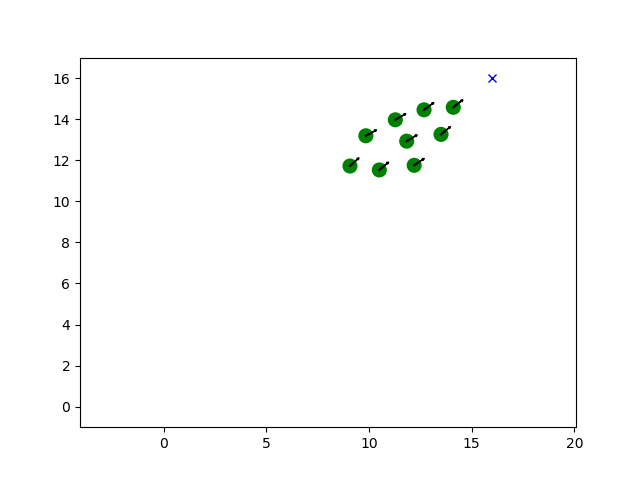
\includegraphics[width=\textwidth]{figures/merge_3.png}
         \caption{after merging}
         \label{fig:merging_c}
     \end{subfigure}
        \caption{Formation merging of two groups}
        \label{fig:merging}
\end{figure}

We quantify the above two formation results in the line chart as \ref{fig:comparison}. We evaluate the compact formation performance by calculating the average distance among all UAVs in each time slice, and the distance between every 2 UAVs are calculated from the center of circle regardless of robot size and safe distance. That is, the shorter the average distance, the more compactly our formation performs. We than simulate a leader-follower based approach where 9 UAVs are set in a 3x3 square formation as our optimal baseline. It can be seen in the graph that the two simulations end up converging to a formation with an average distance around 2.4 to 2.5 (m), and the leader-follower approach maintains its average distance at around 2.2 (m).

\begin{figure}[H]
    \centering
    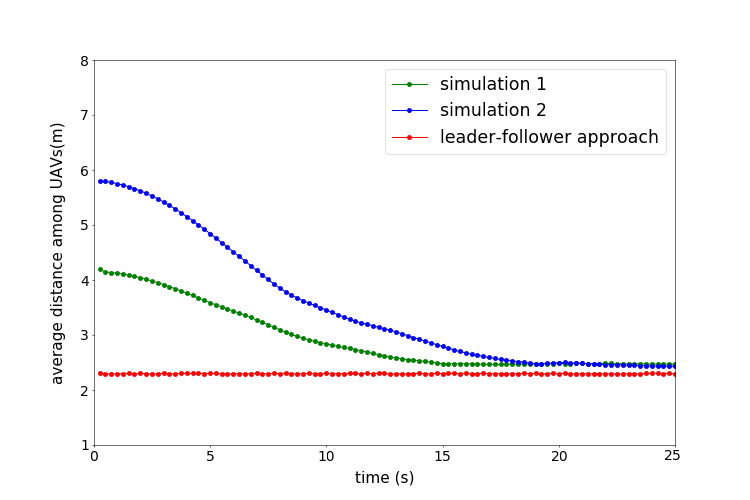
\includegraphics[scale=1]{figures/average_distance_comparison.png}
    \caption{Line chart of the compactness comparison}
    \label{fig:comparison}
\end{figure}

\section{Validation of Comprehensive Performance}
\subsection{Multiple Obstacles Avoidance}
We set up an environment with multiple obstacles dispersed randomly with a radius from 0.2 (m) to 1.5 (m) in the flight space. The goal point is set at (24, 24), and a formation flight for a team is considered to start from the left-down corner. The team consists of six UAVs, which the initial positions are set to (1, 5), (3, 5), (5, 5), (3, 3), (5, 3), (5, 1) respectively, and their predefined trajectories are straight lines toward the goal point.

The result is shown in Figure \ref{fig:trajectory}, where colored-dashed lines denote the trajectories corresponding to each UAV. The group separates in the beginning to avoid the small obstacle placed in (9, 9), and they then merge into a group after passing it. Before reaching the goal point, the split again to dodge a bigger obstacle successfully.

\begin{figure}[H]
    \centering
    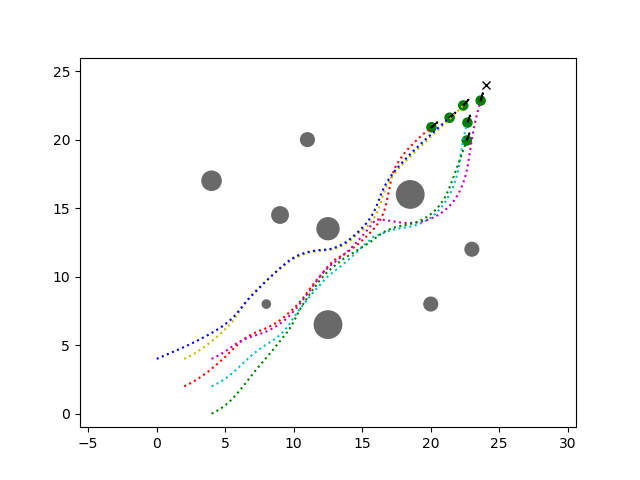
\includegraphics[scale=0.7]{figures/exp1-3.png}
    \caption{Overall trajectories for obstacles avoidance}
    \label{fig:trajectory}
\end{figure}

\subsection{Passing Through a Narrow Passage}
To test the capability of formation compression, we set up a narrow passage for the UAV team to pass through. In the simulation, UAVs should switch the state $flying$ to state $waiting$ before passing through the narrow passage. The result is shown in Figure \ref{fig:narrow}, where a team of 8 UAVs start from the left and the goal point is set on the right. In Figure \ref{fig:narrow}, we use the color for UAVs to identify the states while passing through the passage, where the green UAVs represent the ones in a $flying$ state and the black ones are for the $waiting$ state. It is evident that both sides of the UAVs predict the inter-vehicle collision may occur before entering, and therefore they wait for the other teammates to pass first.

\begin{figure}[H]
    \centering
    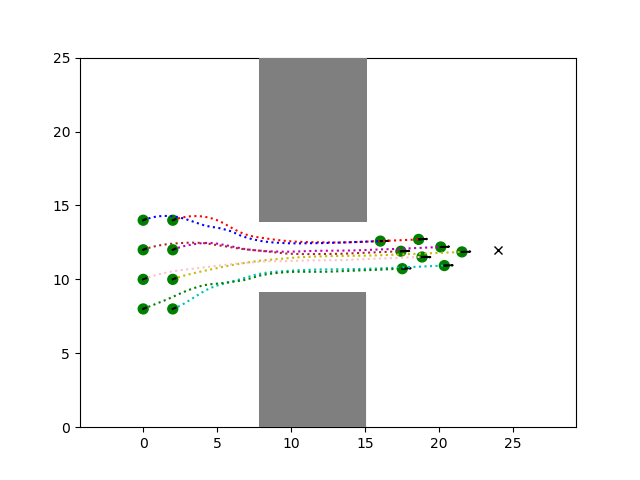
\includegraphics[scale=1]{figures/trail_overall.png}
    \caption{Overall trajectories in a narrow passage}
    \label{fig:narrow}
\end{figure}
\begin{figure}[H]
    \centering
    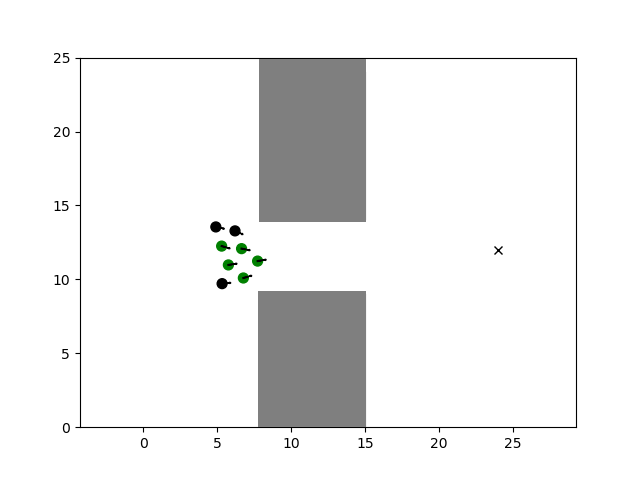
\includegraphics[scale=1]{figures/trail_enter.png}
    \caption{Waiting state validation}
    \label{fig:wait}
\end{figure}

\subsection{Maze-like Environment}
More complex obstacles are placed on testing comprehensive functionality. Due to the limited sensor, UAVs cannot predict the obstacles that might block the direction far away in advance. Our algorithm requires neither leader nor fixed formation so that the team can easily fly in the opposite direction, and find another solution.

Figure \ref{fig:maze} shows that the 6 UAVs are blocked in the beginning after they move for a short distance. Nevertheless, the pioneers invoke the state $navigating$ when there is no available path. On the other hand, the UAVs behind switch the state $flying$ to $waiting$ and wait for their teammates. To prevent deadlock, we preset a time-out variable $clock$. $clock$ is randomly assigned from 2 to 3 seconds for dealing with the synchronize problem. That is, every UAV will start to navigate new paths after the time-out. Finally, it can be seen that the team successfully find another route and fly toward the goal point.

Figure \ref{fig:analysis} shows the analysis of UAV's performance in Figure \ref{fig:maze} from $N = 1$ to $15$, where $N=1$ represents a single UAV which does not require formation coordination. The green line denotes the UAV's average distance, and the red line denotes the total spent time. Since we define $v_{max} = 1m/s$ in the simulation, the
average waiting time when UAVs are being stuck can be analyzed from the difference between both lines. It can be seen that the average distance does not largely affect by the number of UAVs, which shows the stability of our formation coordination algorithm. On the other hand, the total time spent depends on $N$ due to the obstacle that blocks the direction. In the area where UAVs try to find a way out, each UAV switch the state between $waiting$ and $navigating$ to prevent a deadlock, In conclusion, it is similar to a stack(i.e., last-in-first-out structure), and the total time is a linear growth depends on $N$.


\begin{figure}[H]
    \centering
    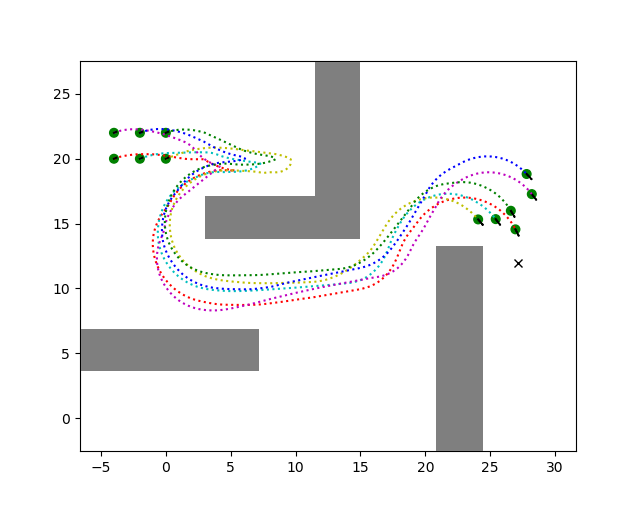
\includegraphics[scale=1]{figures/comprehensive_simulation_2.png}
    \caption{Overall trajectories in a maze-like environment}
    \label{fig:maze}
\end{figure}

\begin{figure}[H]
    \centering
    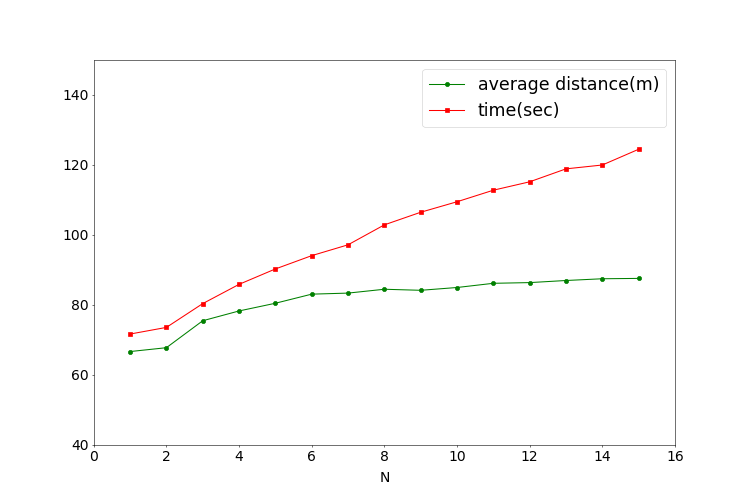
\includegraphics[scale=0.3]{figures/analysis.png}
    \caption{Line chart of the average distance and the total time spent}
    \label{fig:analysis}
\end{figure}

